\documentclass[12pt]{article}         % the type of document and font size (default 10pt)
\usepackage[noae]{Sweave} 
\usepackage{arev}
\usepackage[margin=1.0in]{geometry}   % sets all margins to 1in, can be changed
\usepackage{moreverb}                 % for verbatimtabinput -- LaTeX environment
\usepackage{url}                      % for \url{} command
\usepackage{amssymb}                  % for many mathematical symbols
\usepackage[pdftex]{lscape}           % for landscaped tables
\usepackage{longtable}                % for tables that break over multiple pages

\title{\Huge Title of Coursework \\[0.5in] \large CM3111: Big Data Analysis Coursework \\[2in]}  % to specify title

\author{Eilidh Southren \\[0.25in] Student ID: 1513195\\[3in]}          % to specify author(s)

\date{November 2018}
\begin{document}                      % document begins here
\Sconcordance{concordance:coursework.tex:coursework.Rnw:%
1 19 1 1 2 106 1 1 2 1 0 1 1 3 0 1 2 1 1 1 3 7 0 1 1 6 0 1 2 1 1 1 2 18 %
0 1 2 1 1 1 2 8 0 1 2 2 1 1 2 1 0 2 1 9 0 1 2 3 1 1 6 8 0 1 2 5 1 1 2 1 %
0 1 2 4 0 1 2 1 1 1 8 10 0 1 2 6 1 1 5 7 0 1 2 5 1 1 2 7 0 1 2 1 1 1 3 %
30 0 2 2 4 0 1 2 1 1 1 3 2 0 1 1 5 0 1 1 3 0 1 2 7 1 1 2 1 0 1 2 1 1 3 %
0 2 2 1 0 1 1 1 4 2 0 2 2 4 0 2 2 17 0 1 2 1 1 1 2 8 0 1 2 4 1 1 2 4 0 %
1 2 9 1 1 2 4 0 1 2 7 1 4 0 1 3 4 1 1 5 7 0 1 2 1 1 1 2 17 0 1 2 1 1 1 %
2 8 0 1 2 4 1 1 2 4 0 1 2 7 1 4 0 1 3 2 1 4 0 1 3 2 1 5 0 1 4 4 1 1 2 1 %
0 1 2 1 1 1 3 1 0 2 2 3 0 1 2 1 1 1 2 20 0 1 3 6 1 1 2 4 0 1 2 9 1}



% If .nw file contains graphs: To specify that EPS/PDF graph files are to be 
% saved to 'graphics' sub-folder
%     NOTE: 'graphics' sub-folder must exist prior to Sweave step
%\SweaveOpts{prefix.string=graphics/plot}

% If .nw file contains graphs: to modify (shrink/enlarge} size of graphics 
% file inserted
%         NOTE: can be specified/modified before any graph chunk
\setkeys{Gin}{width=1.0\textwidth}

\maketitle              % makes the title
\pagebreak
\tableofcontents        % inserts TOC (section, sub-section, etc numbers and titles)
%\listoftables           % inserts LOT (numbers and captions)
%\listoffigures          % inserts LOF (numbers and captions)
%                        %     NOTE: graph chunk must be wrapped with \begin{figure}, 
%                        %  \end{figure}, and \caption{}
%%%%%%%%%%%%%%%%%%%%%%%%%%%%%%%%%%%%%%%%%%%%%%%%%%%%%%%%%%%%%%%%%%%%
% Where everything else goes
\pagebreak
\section{How to typeset \textsf{R} code}

If you want to see both the input and output, do this:

\begin{Schunk}
\begin{Sinput}
> runif(10)
\end{Sinput}
\begin{Soutput}
 [1] 0.951700400 0.147350547 0.656194884 0.009407798 0.678570091 0.800007238
 [7] 0.383267459 0.311992274 0.142615642 0.402582072
\end{Soutput}
\end{Schunk}

If you want to see output, but no input, do this:

\begin{Schunk}
\begin{Soutput}
 [1] 0.87171162 0.15202862 0.76866646 0.53133333 0.70905597 0.07119464
 [7] 0.85124164 0.21932358 0.30450789 0.91938220
\end{Soutput}
\end{Schunk}

If you want to see input, but no output, do this:

\begin{Schunk}
\begin{Sinput}
> runif(13)
\end{Sinput}
\end{Schunk}

If you want to run some \textsf{R} code but hide the input/output from the reader then you can do both at the same time:


\bigskip   % leave some empty space (optional)

and you can double-check that it worked later (if you like)

\begin{Schunk}
\begin{Sinput}
> x  # use keep.source=TRUE if you want comments printed
\end{Sinput}
\begin{Soutput}
 [1]  2  3  4  5  6  7  8  9 10 11
\end{Soutput}
\begin{Sinput}
> y
\end{Sinput}
\begin{Soutput}
 [1] 0.4527397 0.7465630 0.3143172 0.6611272 0.4862785 0.6339000 0.7735888
 [8] 0.3827385 0.3238573 0.2071869
\end{Soutput}
\end{Schunk}

If you want to write some \textsf{R} code but not have it evaluated at all then do this:

\begin{Schunk}
\begin{Sinput}
> # whatever you write here must be syntactically correct R code
> runif(1000000000000000000000000)
\end{Sinput}
\end{Schunk}

If you would like to include a figure that's generated completely by \textsf{R} code, then you can do something like the following.

\begin{figure}
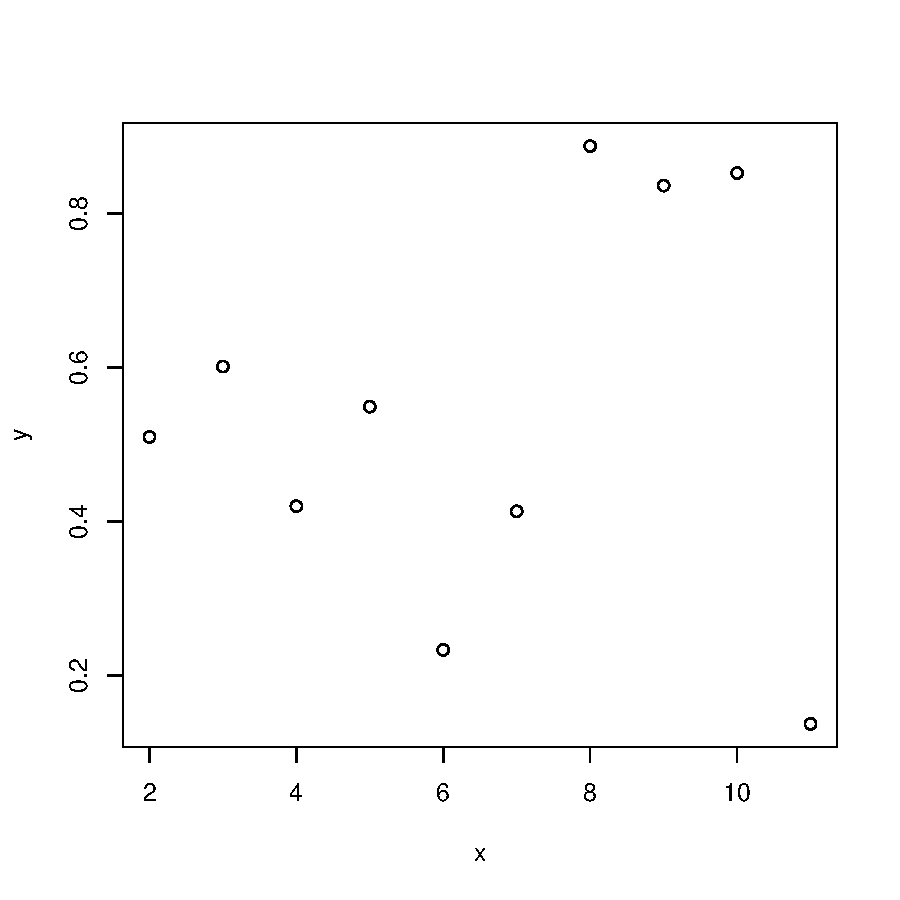
\includegraphics{coursework-007}
\caption{Here is the plot we made}
\end{figure}


Sometimes we would like the output to look like \LaTeX\ output instead of \textsf{R} output.  In that case, do the following.

\begin{Schunk}
\begin{Sinput}
> library(xtable)
> xtable(summary(lm(y ~ x)), caption = "Here is the table we made")
\end{Sinput}
% latex table generated in R 3.5.1 by xtable 1.8-3 package
% Fri Oct 19 15:31:55 2018
\begin{table}[ht]
\centering
\begin{tabular}{rrrrr}
  \hline
 & Estimate & Std. Error & t value & Pr($>$$|$t$|$) \\ 
  \hline
(Intercept) & 0.6693 & 0.1489 & 4.49 & 0.0020 \\ 
  x & -0.0263 & 0.0210 & -1.26 & 0.2446 \\ 
   \hline
\end{tabular}
\caption{Here is the table we made} 
\end{table}\end{Schunk}

\pagebreak 
\section{How to typeset \textsf{R} code}
\pagebreak 
\section{How to typeset \textsf{R} code}


\end{document}

